\documentclass{article}
\usepackage[utf8]{inputenc}
\usepackage{fancyhdr}
\usepackage[margin=1.0in]{geometry}
\usepackage{amsmath}
\usepackage{changepage}
\usepackage{graphicx}
\usepackage[inline]{enumitem} 
\pagestyle{fancy}
\chead{Math 121 - Differentiability}

\begin{document}
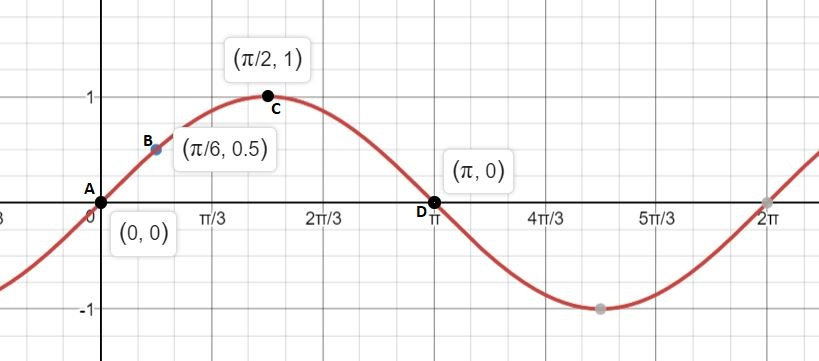
\includegraphics[width=\textwidth]{1.JPG}
\begin{enumerate}
\item This is a graph of the function $f(x) = \sin(x)$. Identify the labeled points in the graph above where the derivative is:\\
\begin{itemize*}
\item $ \frac{\pi}{3} $ \hspace{0.25in}
\item $-1$ \hspace{0.25in}
\item 0 \hspace{0.25in}
\item $1$
\end{itemize*}
\item Sketch functions that fulfill the following requirements:
\begin{itemize}
\item A function that is continuous everywhere, but isn't differentiable at 0.
\item A function that isn't differentiable at 2 and -2.
\item A function whose derivative is always positive.
\item A function whose derivative is always negative.
\end{itemize}
\item Find the derivatives of the following functions using the power rule:
\begin{itemize}
\item $ f(x) = \frac{1}{4}x^2 $, find $f'(x)$
\item $ g(x) = 1 + x + \frac{x^2}{2} + \frac{x^3}{6} + \frac{x^4}{24} $, find $g'(x)$
\item $ y = \sqrt{x}-\frac{1}{\sqrt{x}} $, find $\frac{dy}{dx}$
\item $ x = \frac{5t^2 - 7t^3}{9t^5} $, find $\frac{dx}{dt}$
\end{itemize}
\item Find the first 5 derivatives of each of the functions below.
\begin{itemize}
    \item $\sin(x)$
    \item $\cos(x)$
\end{itemize}
\item What is $\frac{d^{25}}{dx^{25}} \sin(x)$?
\end{enumerate}
\end{document}